\documentclass{article}
\usepackage{jmlr2e}
\usepackage{booktabs}
\firstpageno{1}

\begin{document}

\title{Vector Autoregression (VAR) of Longitudinal Sleep and Self-report Mood Data}

\author{\name Jeff Brozena \email brozena@psu.edu}
\editor{Could use one}
\ShortHeadings{Sleep and Mood}{Jeff Brozena}
\maketitle

\begin{abstract}%

  Self-tracking is one of many behaviors involved in the long-term
  self-management of chronic illnesses. As consumer-grade wearable sensors have
  made the collection of health-related behaviors commonplace, the quality,
  volume, and availability of such data has dramatically improved. This
  exploratory longitudinal N-of-1 study quantitatively assesses four years of
  sleep data captured via the Oura Ring, a consumer-grade sleep tracking device,
  along with self-reported mood data logged using eMood Tracker for iOS. After
  assessing the data for stationarity and computing the appropriate lag-length
  selection, a vector autoregressive (VAR) model was fit along with Granger
  causality tests to assess causal mechanisms within this multivariate time
  series. Oura's nightly sleep quality score shown to Granger-cause
  self-reported presence of depressed mood using a VAR(3) model. 

\end{abstract}

\hypertarget{introduction}{%
\section{Introduction}\label{introduction}}

Long-term self-management of chronic illnesses such as bipolar disorder require
persistent awareness of illness state over long periods of time and at varying
time scales \citep{murnane2016SelfmonitoringPracticesAttitudes,
morton2018TakingBackReins, majid2022ExploringSelftrackingPractices}. Remaining
consistently aware of key indicators signalling the onset of a chronic condition
allow individuals a chance at early intervention to reduce the severity of a
givene episode. For example, an individual may modify behavior, engage their
health practitioners, or adjust medication dosage. However nuanced, bipolar
disorder is an illness that often degrades an individual's self-awareness and
capacity for self-monitoring during symptomatic periods.

In the context of this specific illness, a volume of prior work has demonstrated
the vital role of sleep in order to promote mood stability and prevent
symptomatic episodes
\citep{harveySleep2009,murrayCircadian2010,gruberSleep2011}. Although the
particulars of this topic fall beyond the scope of this paper, these nuanced
relationships may in fact be self-reinforcing and bidirectional --- poor sleep
may lead to episodic onset, which may also lead to worsening (or shortening)
sleep bouts.

Given the importance of sleep in the ongoing management of this illness,
accurate consumer-grade alternatives to polysomnography (considered the gold
standard of sleep tracking) have emerged over the last few years. Indeed,
comparatively inexpensive sleep tracking technologies like the Oura Ring have
dramatically improved the quality of information that can be used to augment and
inform these self-monitoring activities. Objective sensor-based tracking
technology can be complemented with subjective self-report measures in order to
form a more complete picture of physical and mental health across time. Given
the aforementioned interplay of sleep and mood, this combination of subjective
and objective tracking creates the possibility of longitudinal analysis --- and
potentially deepens one's capacity for self-awareness.

Following four years of consistent sleep and mood tracking, I sought to more
formally interpret the data I had collected to quantify what I had previously
intuited: that certain mood states could be understood (and potentially even
predicted) by recent sleep trends. Indeed, this intuition has been demonstrated
quantitatively in existing literature \citep{boseVector2017,
moshePredicting2021, jafarlouObjective2023}. As this work also demonstrates,
combining data from consumer wearable technology and subjective self-report logs
allows for a more comprehensive picture of health.

I will first describe the vector autoregression (VAR) method and subsequent
tests, namely the Granger causality test and an impulse response analysis, that
were performed to achieve these goals.

First, I will describe the methods used to achieve these goals, providing an
overview of vector autoregression, Granger causality, and impulse response
functions. Next, I will detail the findings of these methods on the dataset.
This work concludes with a discussion of the methods and their potential
applications in future work.

\hypertarget{methods}{%
\section{Problem setup}\label{methods}}

A multivariate time series analysis was performed using a vector autoregressive
(VAR) model fit using ordinary least squares. An optimal lag order was first
obtained using a combination of Akaike Information Criterion (AIC), Bayesian
Information Criterion (BIC), Hannan-Quinn Information Criterion (HQIC), and
final prediction error (FPE). After fitting a VAR(3) model on the multiple time
series data (outlined below), a Granger causality test was performed in order to
assess the predictive relationships between variables. Finally, an impulse
response analysis was plotted to further explore the temporal relationships
between variables, specifically between sleep, heartrate variability, and
self-reported mood. I will outline these analysis steps in greater detail in the
sections that follow.

\hypertarget{vector-autoregression}{%
\subsection{Vector Autoregression}\label{vector-autoregression}}

\citep{seabold2010statsmodels}

\citep{lutkepohlNew2005}

Pellentesque est dolor, porttitor sed est at, interdum elementum diam.
Sed bibendum enim ante. Sed vestibulum diam at arcu tincidunt, quis
aliquet dui lobortis. Donec ultricies ipsum ac eros sodales, et placerat
massa suscipit. Etiam luctus arcu quis blandit auctor. In ultricies nisi
dignissim enim finibus, sit amet fringilla dolor facilisis. Donec sit
amet lectus eu lorem porta vehicula. Cras vel ex vehicula, fermentum mi
sed, aliquet ante. Maecenas gravida odio eget mi iaculis, non
scelerisque tortor ornare.

Nam eu varius lacus. Aliquam ultricies diam id nibh vehicula
consectetur. Nullam euismod felis a aliquam iaculis. Quisque nibh enim,
varius a porta lacinia, lobortis vel nisl. Vestibulum molestie nunc et
luctus dapibus. Phasellus eget lectus id ligula sollicitudin consequat
et a nunc. Class aptent taciti sociosqu ad litora torquent per confaubia
nostra, per inceptos himenaeos. Praesent eros magna, tempor vitae justo
condimentum, consectetur fermentum magna. Praesent commodo mauris non
massa pulvinar, vitae blandit sem eleifend. Vivamus varius eu nisi in
volutpat. Aliquam scelerisque nunc vel orci euismod suscipit.

Nam eu varius lacus. Aliquam ultricies diam id nibh vehicula
consectetur. Nullam euismod felis a aliquam iaculis. Quisque nibh enim,
varius a porta lacinia, lobortis vel nisl. Vestibulum molestie nunc et
luctus dapibus. Phasellus eget lectus id ligula sollicitudin consequat
et a nunc. Class aptent taciti sociosqu ad litora torquent per confaubia
nostra, per inceptos himenaeos. Praesent eros magna, tempor vitae justo
condimentum, consectetur fermentum magna. Praesent commodo mauris non
massa pulvinar, vitae blandit sem eleifend. Vivamus varius eu nisi in
volutpat. Aliquam scelerisque nunc vel orci euismod suscipit.

\hypertarget{granger-causality}{%
\subsection{Granger Causality}\label{granger-causality}}

Nunc eget risus nec odio commodo feugiat nec ac arcu. Maecenas laoreet
lorem ut mi tristique ultricies. Maecenas lacinia fermentum euismod.
Praesent quis ornare urna. Orci varius natoque penatibus et magnis dis
parturient montes, nascetur ridiculus mus. Nunc non ornare risus. Nunc
vulputate risus a dapibus eleifend. Aenean justo lacus, dignissim eget
gravida sed, laoreet eu neque. Vivamus volutpat risus non ligula feugiat
sollicitudin. Ut nec porttitor ipsum.

Nulla lobortis neque blandit dui tristique placerat. Cras a tempor leo,
nec vulputate libero. Vivamus efficitur ipsum sit amet enim pretium,
eget consequat turpis luctus. Aenean mattis velit vitae odio lobortis,
ut sodales augue posuere. Pellentesque habitant morbi tristique senectus
et netus et malesuada fames ac turpis egestas. Vestibulum ac accumsan
eros, a mattis lacus. Sed in lectus felis. Fusce quis dui odio. Integer
tincidunt vitae tortor a tempus. Nam venenatis eros rutrum quam
tristique finibus. Nullam varius vel massa at iaculis. Morbi
condimentum, loremh non tempus auctor, mauris arcu tempus libero, ac
venenatis odio enim at odio. Maecenas egestas sit amet lorem in aliquet.
Aenean nec eros ante.

\hypertarget{impulse-response-analysis}{%
\subsection{Impulse Response Analysis}\label{impulse-response-analysis}}

Nulla lobortis neque blandit dui tristique placerat. Cras a tempor leo,
nec vulputate libero. Vivamus efficitur ipsum sit amet enim pretium,
eget consequat turpis luctus. Aenean mattis velit vitae odio lobortis,
ut sodales augue posuere. Pellentesque habitant morbi tristique senectus
et netus et malesuada fames ac turpis egestas. Vestibulum ac accumsan
eros, a mattis lacus. Sed in lectus felis. Fusce quis dui odio. Integer
tincidunt vitae tortor a tempus. Nam venenatis eros rutrum quam
tristique finibus. Nullam varius vel massa at iaculis. Morbi
condimentum, loremh non tempus auctor, mauris arcu tempus libero, ac
venenatis odio enim at odio. Maecenas egestas sit amet lorem in aliquet.
Aenean nec eros ante.


\hypertarget{results}{%
\section{Experimental Results}\label{results}}

Nullam non risus augue. Nunc commodo pharetra eros, non condimentum sem
ultrices ut. Nunc pharetra enim eget commodo pharetra. Pellentesque
ultricies placerat bibendum. Donec ligula ex, rhoncus vitae finibus
eget, malesuada in massa. Nam porta varius ex ac ullamcorper. Vivamus
eget neque sit amet ex semper elementum. Aliquam erat volutpat.
Pellentesque habitant morbi tristique senectus et netus et malesuada
fames ac turpis egestas. Morbi semper ultricies ex, in eleifend erat
congue a. Nunc et venenatis sapien. Aliquam vel lectus scelerisque,
pellentesque enim ac, sagittis erat. Praesent molestie, velit eget
pretium venenatis, est nisl rutrum orci, ut placerat leo odio in nulla.
Sed bibendum nunc libero, in vestibulum metus hendrerit at.

\hypertarget{dataset-description}{%
\subsection{Dataset Description}\label{dataset-description}}

The sleep score dataset was created using the second- and third-generation Oura
Ring. As detailed in Table \ref{Sleep}, my use of the Oura Ring was consistent across
time. The proprietary Oura sleep score is on a scale of 1 to 100 and
incorporates a variety of sensor-based measures (i.e., heartrate variability,
resting heartrate, body temperature) across time. Although the specifics of this
algorithm are not public, the Oura Ring has been found to produce
accurate measures of sleep timing and heartrate variability when compared
against polysomnography \citep{dezambottiSleep2019}. The dataset contains 1,455
nights of sleep bout data occuring between February, 2019 and March, 2023.

\begin{table}[ht]
  \centering
  \begin{tabular}{lr}
  \toprule
     & \textbf{Value}\\ \midrule
      Total nights & 1455 \\
      Missing nights & 1 \\
      Mean & 73.82 \\
      SD & 12.36 \\
      Max & 97.00 \\
      Min & 30.00 \\
   \bottomrule
  \end{tabular}
\caption{Descriptive statistics of Oura Ring sleep score data}
\label{Sleep}
\end{table}

Aliquam tristique, sem id venenatis pellentesque, elit ante auctor arcu,
ac commodo tellus ante vel massa. Praesent placerat tristique tellus sed
elementum. Etiam vehicula dolor non libero blandit, eu scelerisque felis
pulvinar. Ut ac bibendum ante. Integer consequat, nisi in placerat
dictum, nibh tellus feugiat est, id tristique risus magna venenatis
lectus. Nulla viverra nulla mi, in feugiat velit pharetra dictum. Proin
id viverra mauris. Morbi a pellentesque nisl, at volutpat ligula. Donec
tristique facilisis felis, et euismod mauris. Suspendisse ac massa quis
augue pharetra vestibulum ac ut mi. Phasellus efficitur dignissim nisl.
Vivamus ornare ex vel dui rutrum convallis. Sed nec urna fermentum augue
facilisis ultricies.

\begin{table}[ht]
    \centering
    \begin{tabular}{ll}
    \toprule
        \textbf{EMA Categories} & \textbf{Count} \\ \midrule
        irritable & 100 \\
        anxious & 88  \\
        depressed & 103  \\
        elevated & 48  \\
        \bottomrule
    \end{tabular}
\caption{Count of days where EMA item contains a non-zero value}
\label{EMA}
\end{table}


Nam eu varius lacus. Aliquam ultricies diam id nibh vehicula
consectetur. Nullam euismod felis a aliquam iaculis. Quisque nibh enim,
varius a porta lacinia, lobortis vel nisl. Vestibulum molestie nunc et
luctus dapibus. Phasellus eget lectus id ligula sollicitudin consequat
et a nunc. Class aptent taciti sociosqu ad litora torquent per confaubia
nostra, per inceptos himenaeos. Praesent eros magna, tempor vitae justo
condimentum, consectetur fermentum magna. Praesent commodo mauris non
massa pulvinar, vitae blandit sem eleifend. Vivamus varius eu nisi in
volutpat. Aliquam scelerisque nunc vel orci euismod suscipit.


\hypertarget{stationarity-decomposition-and-autocorrelation}{%
\subsection{Stationarity, Decomposition, and
Autocorrelation}\label{stationarity-decomposition-and-autocorrelation}}

Sed ut lobortis ligula. Nunc vel justo cursus, consequat lectus vel,
accumsan libero. Etiam lectus nisl, varius in feugiat nec, varius id
ligula. Fusce scelerisque pharetra nisl. Maecenas in finibus nisl, in
sagittis dolor. Fusce dictum cursus condimentum. Nullam posuere mauris
vel odio pulvinar auctor. Nullam ante tellus, semper non scelerisque et,
faucibus quis urna. Duis pulvinar metus vel eleifend aliquet. Aenean
cursus nunc vitae porttitor malesuada.

\begin{figure}[h]
\centering
  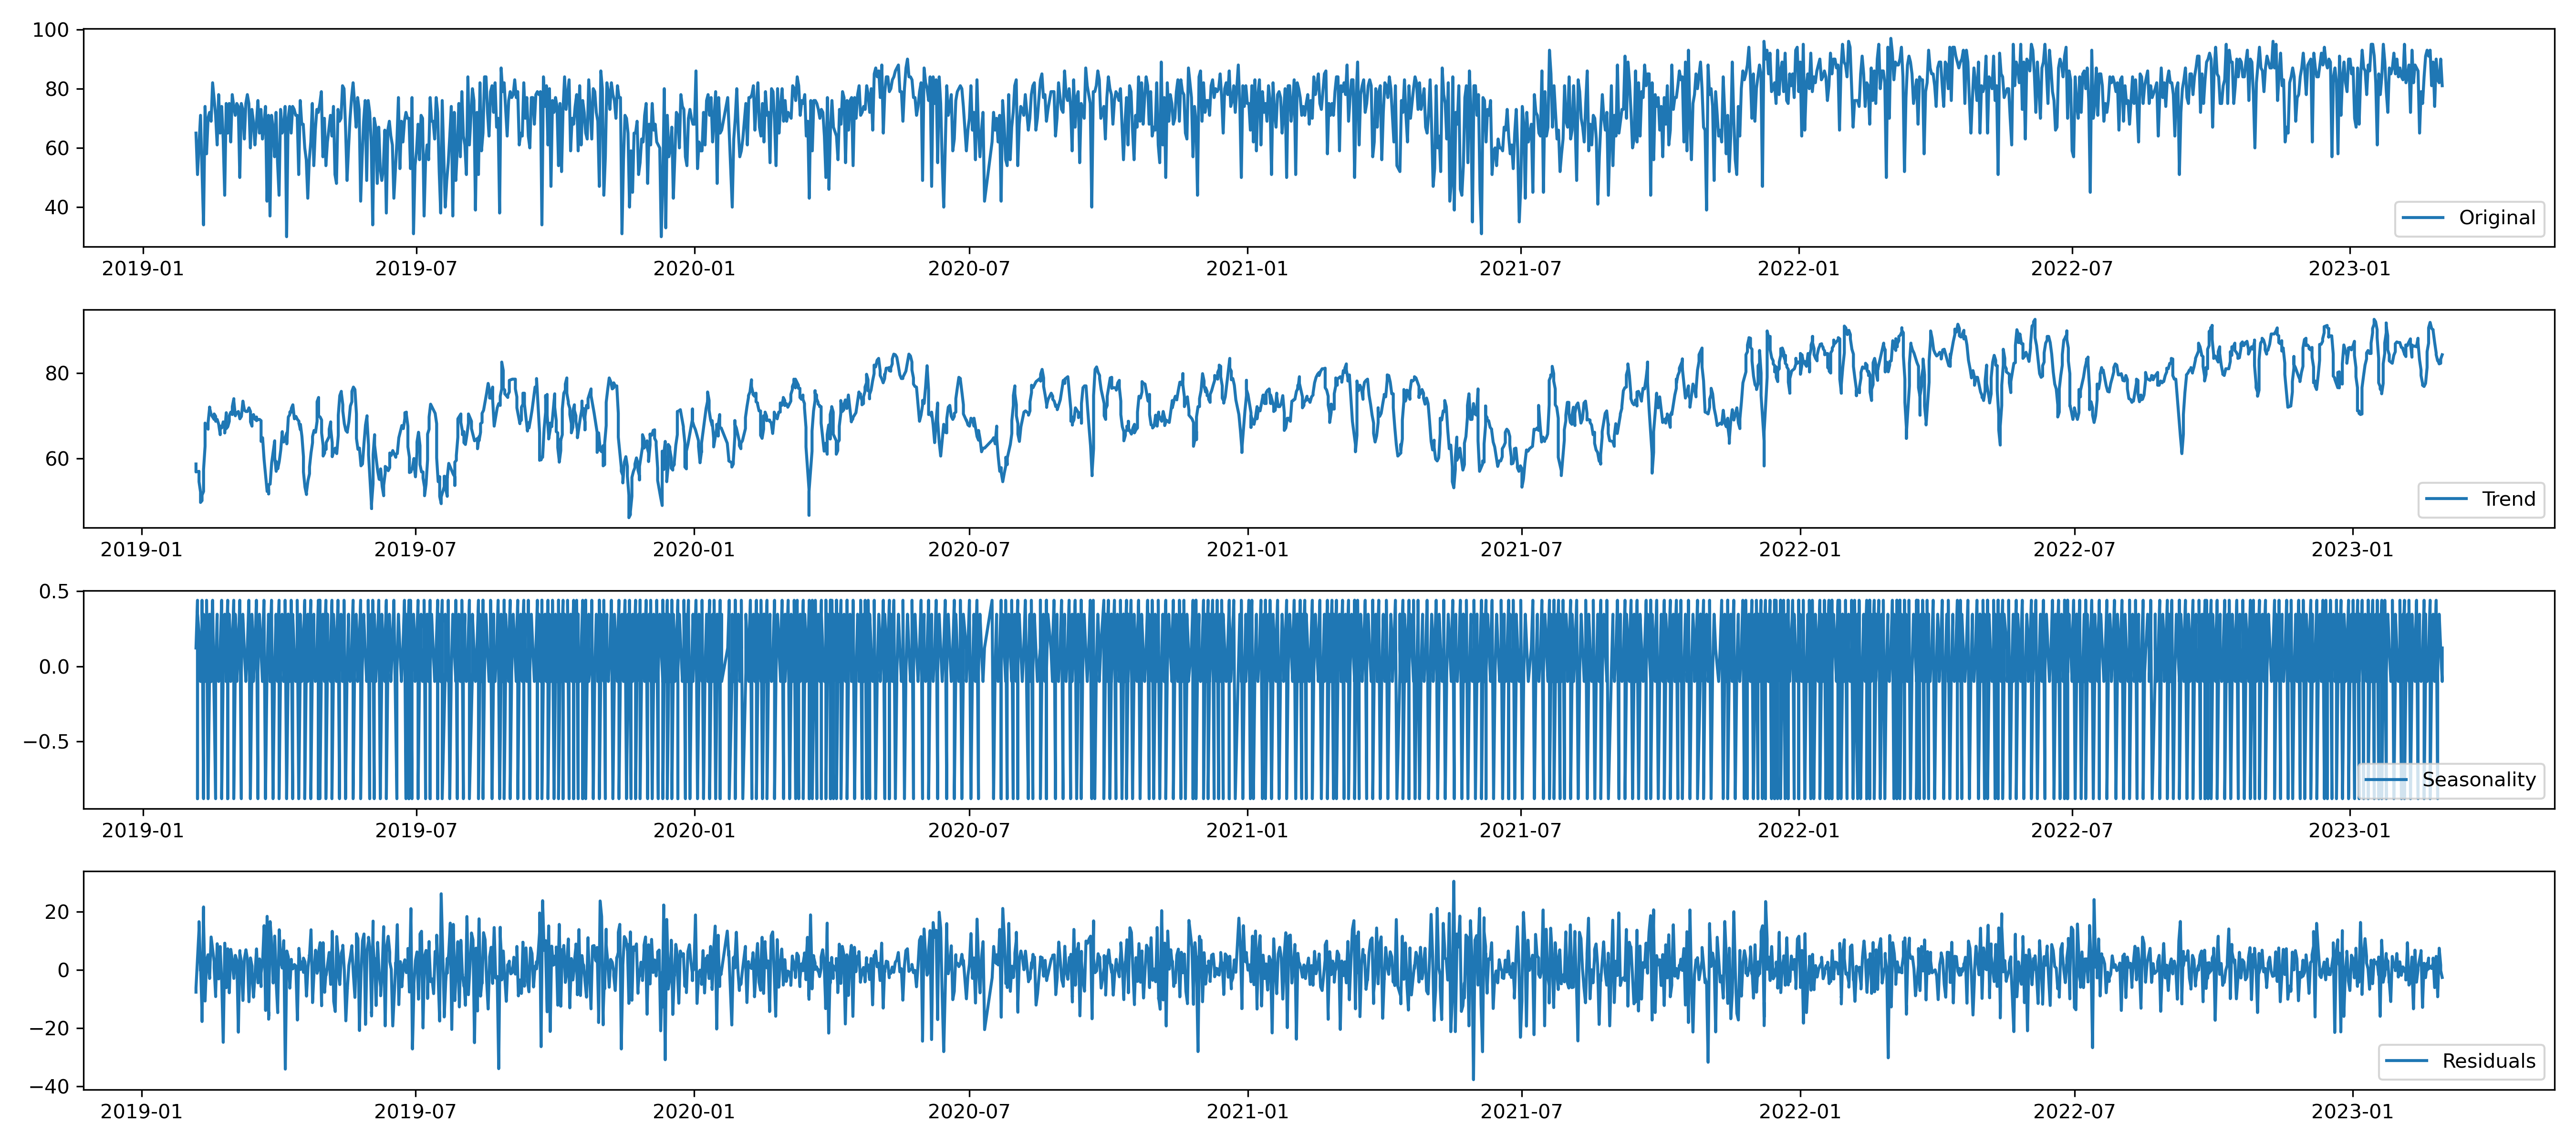
\includegraphics[width=0.8\columnwidth]{/Users/jab/Library/Mobile Documents/com~apple~CloudDocs/PSU/Courses/2023 Spring/STAT508/project/notebooks/plots/decomposition.png}
\caption{Decomposition of sleep time series}
\end{figure}

Sed ut lobortis ligula. Nunc vel justo cursus, consequat lectus vel,
accumsan libero. Etiam lectus nisl, varius in feugiat nec, varius id
ligula. Fusce scelerisque pharetra nisl. Maecenas in finibus nisl, in
sagittis dolor. Fusce dictum cursus condimentum. Nullam posuere mauris
vel odio pulvinar auctor. Nullam ante tellus, semper non scelerisque et,
faucibus quis urna. Duis pulvinar metus vel eleifend aliquet. Aenean
cursus nunc vitae porttitor malesuada.

\begin{figure}[h]
\centering
  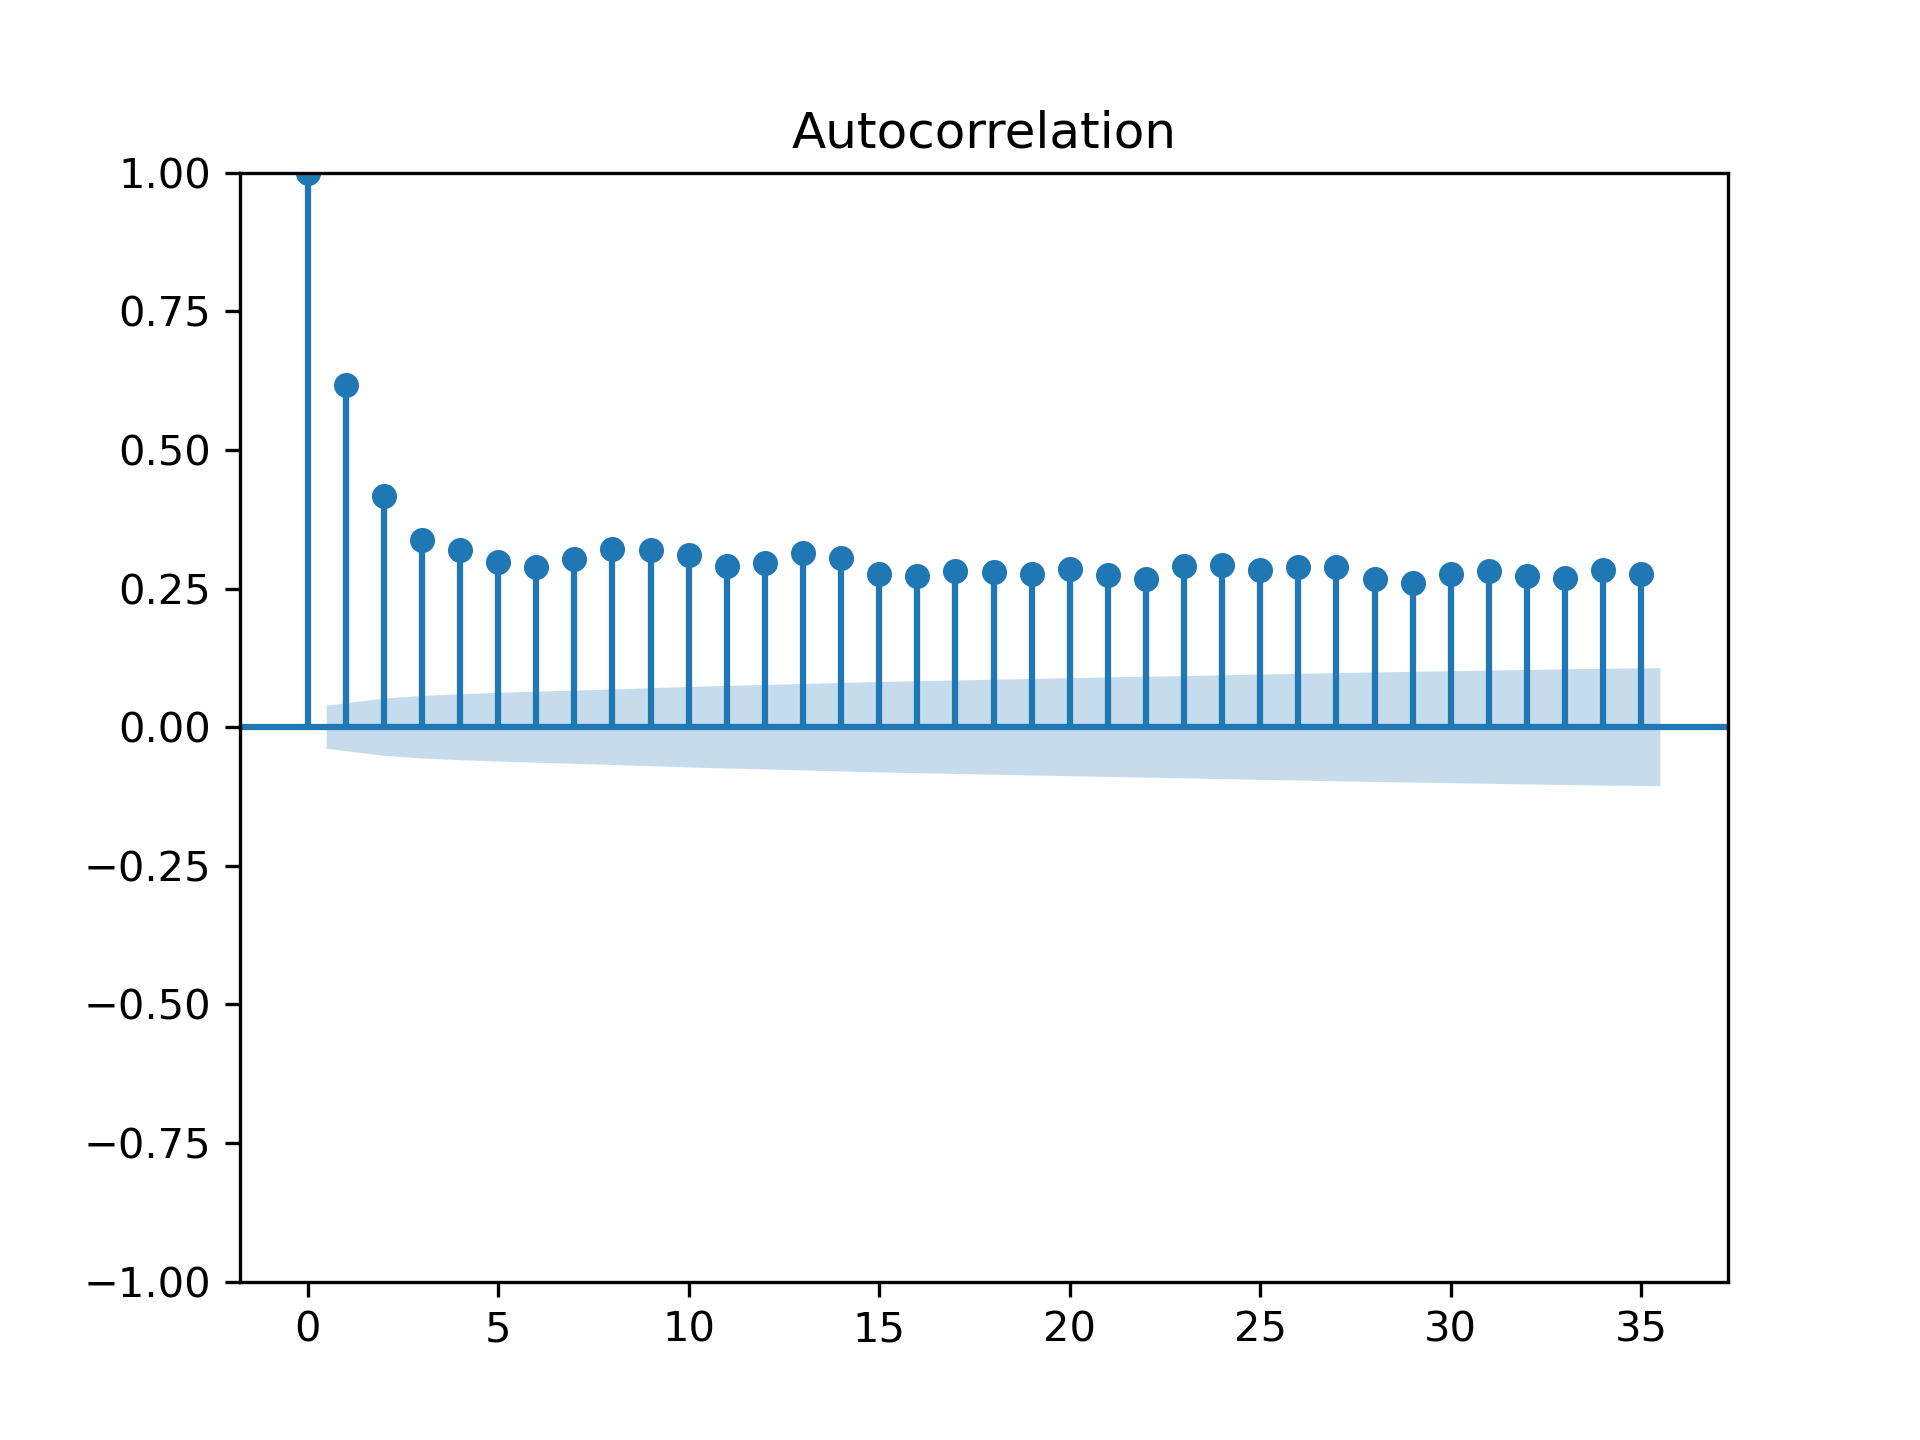
\includegraphics[scale=0.5]{/Users/jab/Library/Mobile Documents/com~apple~CloudDocs/PSU/Courses/2023 Spring/STAT508/project/notebooks/plots/acf.png}
\caption{Autocorrelation of sleep time series}
\end{figure}

Sed ut lobortis ligula. Nunc vel justo cursus, consequat lectus vel,
accumsan libero. Etiam lectus nisl, varius in feugiat nec, varius id
ligula. Fusce scelerisque pharetra nisl. Maecenas in finibus nisl, in
sagittis dolor. Fusce dictum cursus condimentum. Nullam posuere mauris
vel odio pulvinar auctor. Nullam ante tellus, semper non scelerisque et,
faucibus quis urna. Duis pulvinar metus vel eleifend aliquet. Aenean
cursus nunc vitae porttitor malesuada.

\begin{figure}[h]
\centering
  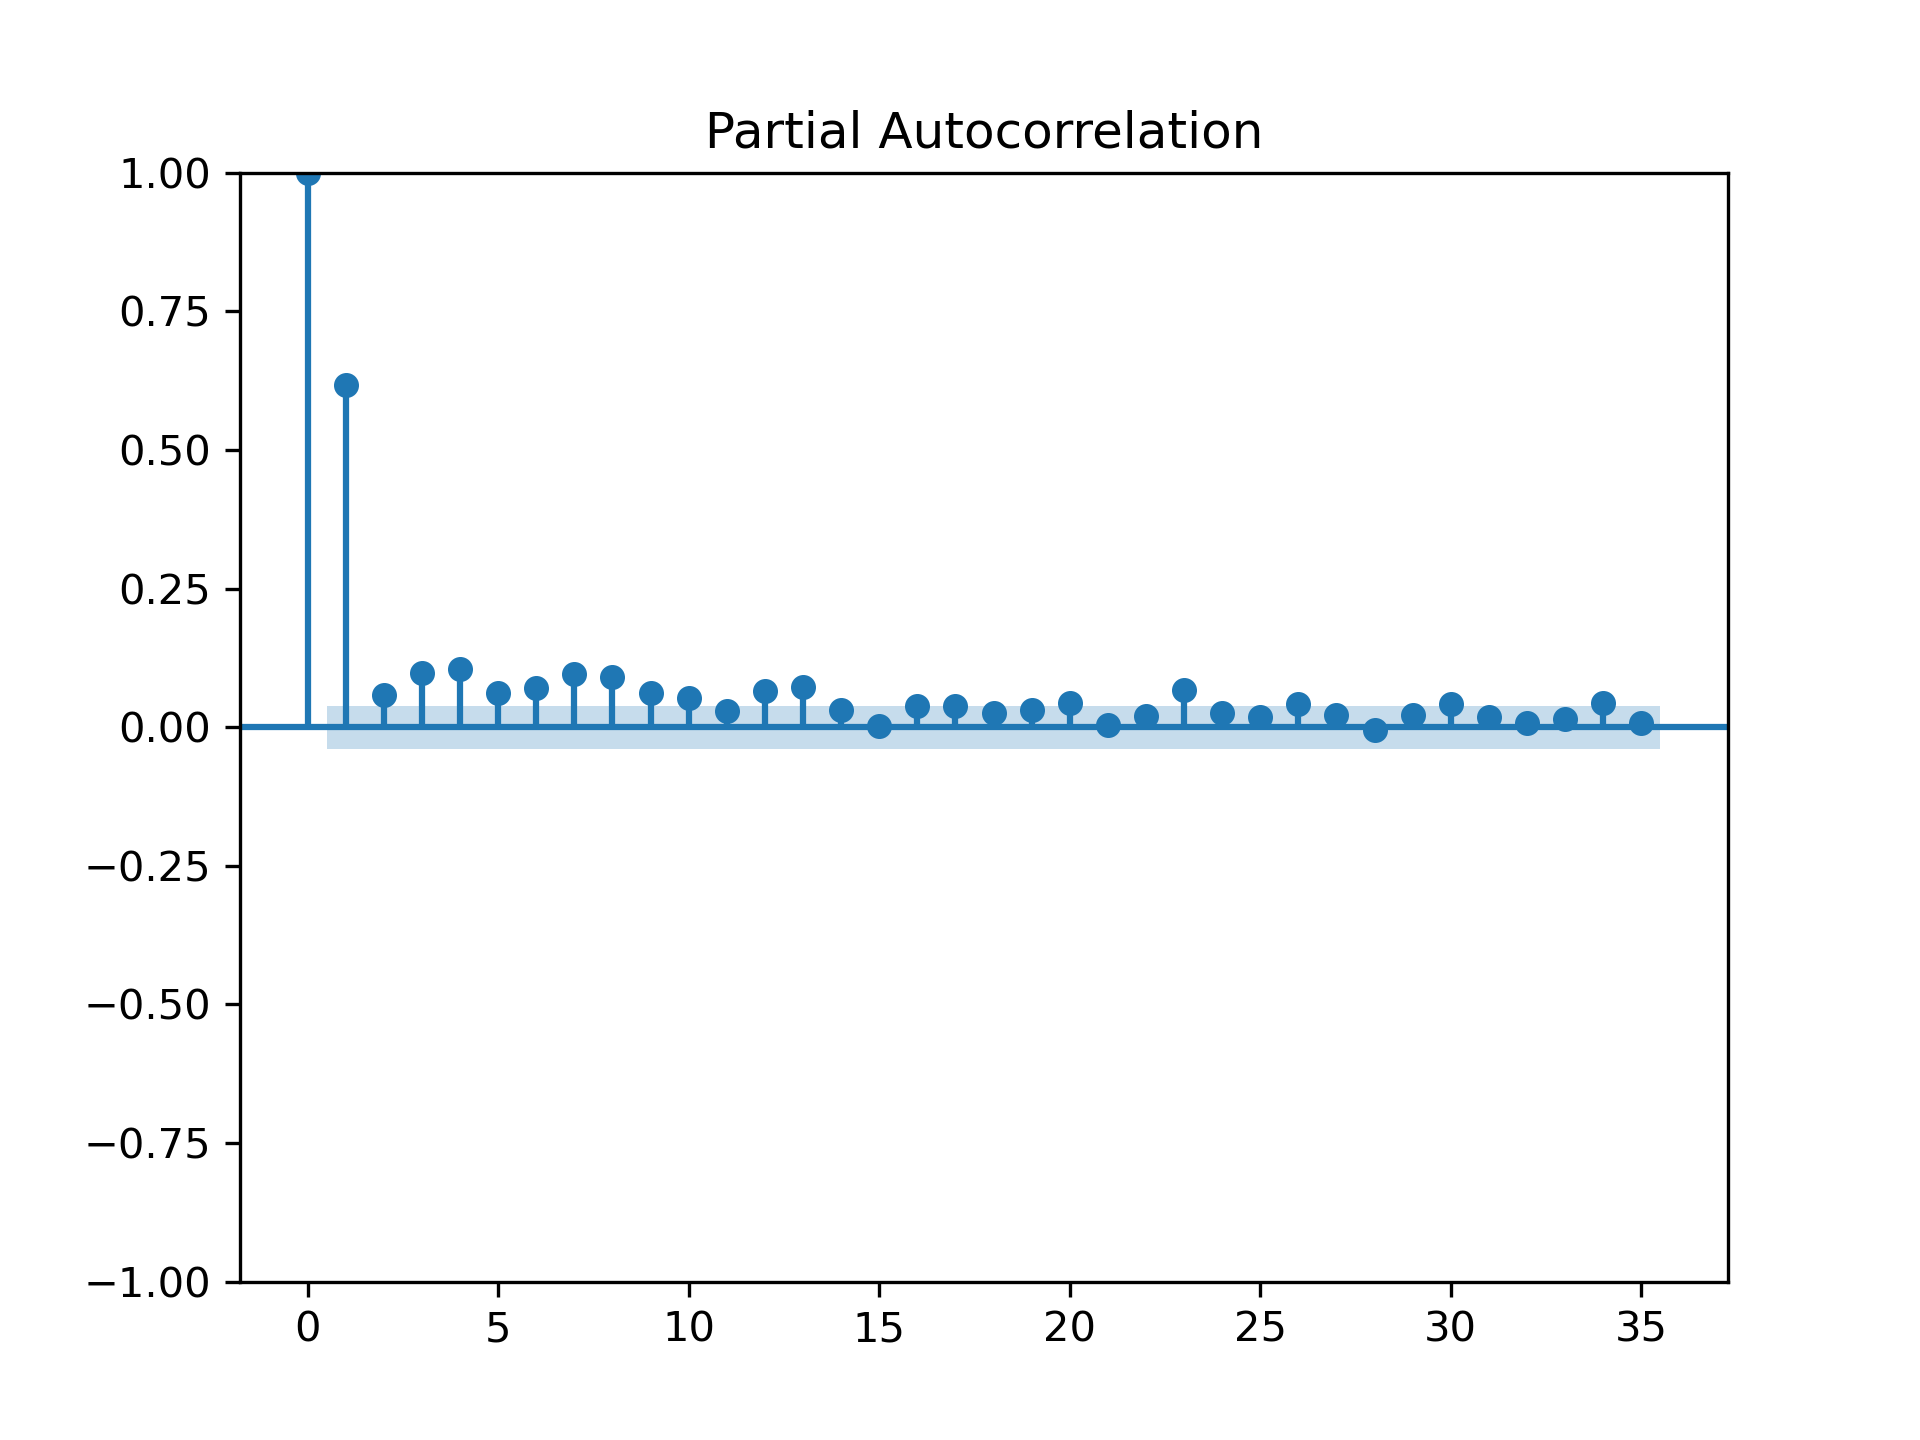
\includegraphics[scale=0.5]{/Users/jab/Library/Mobile Documents/com~apple~CloudDocs/PSU/Courses/2023 Spring/STAT508/project/notebooks/plots/pacf.png}
\caption{Partial autocorrelation of sleep time series}
\end{figure}

\hypertarget{lag-order-selection}{%
\subsection{Lag Order Selection}\label{lag-order-selection}}

In congue tristique fermentum. Morbi eleifend tortor justo, sed iaculis
ante posuere vitae. Quisque sagittis ex sit amet mi sollicitudin tempor
vel in ligula. Morbi porta tincidunt diam, non accumsan lorem maximus
eget. Orci varius natoque penatibus et magnis dis parturient montes,
nascetur ridiculus mus. Sed ut tristique leo, eu facilisis massa.
Maecenas sed nibh hendrerit, rutrum ipsum sit amet, tempus velit. Ut
venenatis dolor nisi, vel egestas est convallis ut. Nulla facilisi.
Aenean vestibulum malesuada eleifend. Sed pulvinar elementum maximus.
Fusce vulputate justo vel est accumsan luctus. Nulla rhoncus nisi at
lacus scelerisque, et pharetra elit interdum. Donec non ante ac nulla
commodo euismod a et neque.

\begin{table}[ht]
    \centering
    \begin{tabular}{lllll}
      \toprule
        ~ & \textbf{AIC} & \textbf{BIC} & \textbf{FPE} & \textbf{HQIC} \\ \midrule
        \textbf{0} & 7.314 & 7.342 & 1501. & 7.325 \\ 
        \textbf{1} & 6.080 & 6.279* & 436.9 & 6.155* \\ 
        \textbf{2} & 6.035 & 6.404 & 417.7 & 6.175 \\ 
        \textbf{3} & 6.028* & 6.568 & 414.9* & 6.233 \\ 
        \textbf{4} & 6.055 & 6.765 & 426.1 & 6.324 \\ 
        \textbf{5} & 6.056 & 6.936 & 426.6 & 6.390 \\ 
        \textbf{6} & 6.066 & 7.118 & 431.2 & 6.465 \\ 
        \textbf{7} & 6.071 & 7.293 & 433.3 & 6.534 \\ 
        \textbf{8} & 6.104 & 7.496 & 447.6 & 6.631 \\ 
        \textbf{9} & 6.131 & 7.694 & 460.4 & 6.724 \\ 
        \textbf{10} & 6.130 & 7.863 & 459.6 & 6.787 \\ 
        \textbf{11} & 6.129 & 8.032 & 459.5 & 6.851 \\ 
        \textbf{12} & 6.158 & 8.232 & 473.0 & 6.944 \\ 
        \textbf{13} & 6.177 & 8.421 & 482.2 & 7.028 \\ 
        \textbf{14} & 6.201 & 8.616 & 494.2 & 7.117 \\ 
        \textbf{15} & 6.213 & 8.798 & 500.3 & 7.193 \\ \bottomrule
    \end{tabular}
    \caption{VAR Order Selection (* highlights the minimum)}
    \label{VAROrderSelection}
\end{table}

Cras pretium imperdiet sem id euismod. In blandit pharetra urna. Integer
molestie eleifend ex, nec tincidunt sapien ullamcorper sit amet. Fusce
dictum purus elit, ut sagittis diam viverra nec. Vestibulum erat felis,
placerat ac ligula eu, dictum lacinia lacus. Maecenas mollis augue sem,
sit amet tincidunt ex fringilla ac. Pellentesque vel metus ipsum. Sed
sit amet nisi vitae tellus consectetur vulputate. Proin aliquam quam at
purus tincidunt, ut pharetra ante posuere. Morbi viverra lacinia leo, ac
malesuada eros aliquam vitae. Vivamus vitae nisl dictum, laoreet nisi
sed, dapibus odio.

\hypertarget{vector-autoregression-model}{%
\subsection{Vector Autoregression
Model}\label{vector-autoregression-model}}

Sed id feugiat tortor. Duis arcu lorem, rutrum ut nunc quis, bibendum
mollis metus. In pulvinar ut mauris in malesuada. Curabitur eu massa
aliquam, laoreet dui maximus, porta tellus. Aliquam erat volutpat. Proin
quis lectus nisl. Mauris sagittis bibendum elit eu accumsan. Aliquam ut
dui faucibus, dictum magna id, venenatis metus. Mauris ex mi, tempor vel
nunc eu, placerat placerat nunc. Cras facilisis varius bibendum. Sed
sollicitudin vel sem in maximus. Aenean aliquam sem ac arcu lacinia,
vitae bibendum mauris malesuada. Praesent ac imperdiet erat. Maecenas
tincidunt sed sem ac porta. Phasellus in justo orci.

\begin{table}[ht]
    \centering
    \begin{tabular}{lllll}
      \toprule\
        ~ & \textbf{coefficient} & \textbf{std. error} & \textbf{t-stat} & \textbf{prob} \\ \midrule
        \textbf{const} & 33.675538 & 2.896460 & 11.626 & 0.000 \\ 
        \textbf{L1.score} & 0.507601 & 0.031112 & 16.315 & 0.000 \\ 
        \textbf{L1.average\_hrv} & -0.050172 & 0.022424 & -2.237 & 0.025 \\ 
        \textbf{L1.anxious} & -0.078201 & 0.494593 & -0.158 & 0.874 \\ 
        \textbf{L1.depressed} & 0.615468 & 0.457538 & 1.345 & 0.179 \\ 
        \textbf{L1.irritable} & -0.015195 & 0.457422 & -0.033 & 0.973 \\ 
        \textbf{L1.elevated} & -0.150473 & 0.729563 & -0.206 & 0.837 \\ 
        \textbf{L2.score} & -0.020902 & 0.034834 & -0.600 & 0.548 \\ 
        \textbf{L2.average\_hrv} & -0.027687 & 0.022370 & -1.238 & 0.216 \\ 
        \textbf{L2.anxious} & 0.178654 & 0.540249 & 0.331 & 0.741 \\ 
        \textbf{L2.depressed} & \textbf{1.427585} & 0.490653 & 2.910 & \textbf{0.004} \\ 
        \textbf{L2.irritable} & -0.634113 & 0.500474 & -1.267 & 0.205 \\ 
        \textbf{L2.elevated} & -0.164427 & 0.771205 & -0.213 & 0.831 \\ 
        \textbf{L3.score} & 0.117166 & 0.031157 & 3.760 & 0.000 \\ 
        \textbf{L3.average\_hrv} & -0.023210 & 0.022319 & -1.040 & 0.298 \\ 
        \textbf{L3.anxious} & 0.003463 & 0.492368 & 0.007 & 0.994 \\ 
        \textbf{L3.depressed} & 0.152999 & 0.458520 & 0.334 & 0.739 \\ 
        \textbf{L3.irritable} & 0.406833 & 0.457032 & 0.890 & 0.373 \\ 
        \textbf{L3.elevated} & -0.805440 & 0.732522 & -1.100 & 0.272 \\ \bottomrule
    \end{tabular}
    \caption{VAR results for equation score}
    \label{VAR Score Results}
\end{table}

Vestibulum sit amet faucibus purus. Proin ornare nisi et purus
pellentesque mollis. Mauris aliquet metus sed sem blandit, quis accumsan
justo blandit. Donec vitae lectus commodo, placerat tellus sed, interdum
ex. Suspendisse potenti. Suspendisse tincidunt, enim in convallis
sollicitudin, metus orci facilisis ex, non tristique nunc est ac magna.
Aenean ut lorem interdum dui dictum venenatis. Nullam hendrerit placerat
mauris, et tempor neque convallis vitae. Pellentesque vitae ligula id
elit hendrerit dapibus. Suspendisse lobortis, dui id ultrices viverra,
lorem arcu ornare dui, faucibus vehicula tortor erat sed ex. Morbi ac
dolor ut nunc fringilla facilisis nec lobortis urna. Nullam ac tempus
turpis.

\hypertarget{granger-causality-1}{%
\subsection{Granger Causality}\label{granger-causality-1}}

\begin{table}[ht]
    \centering
    \begin{tabular}{llllll}
    \toprule
        \textbf{Causal Variable} & \textbf{Variable} & \textbf{Test statistic} & \textbf{Critical value} & \textbf{p-value} & \textbf{df} \\ \midrule
        average\_hrv & depressed & 1.541 & 2.606 & 0.202 & (3, 6234) \\ 
        average\_hrv & anxious & 0.3879 & 2.606 & 0.762 & (3, 6234) \\ 
        average\_hrv & irritable & 0.8046 & 2.606 & 0.491 & (3, 6234) \\ 
        average\_hrv & elevated & 0.6640 & 2.606 & 0.574 & (3, 6234) \\ 
        \textbf{score} & \textbf{depressed} & 5.155 & 2.606 & \textbf{0.001} & (3, 6234) \\ 
        score & anxious & 2.432 & 2.606 & 0.063 & (3, 6234) \\ 
        score & irritable & 1.311 & 2.606 & 0.269 & (3, 6234) \\ 
        score & elevated & 0.7891 & 2.606 & 0.500 & (3, 6234) \\ \bottomrule
    \end{tabular}
    \caption{Granger Causality Test for HRV and Sleep Score}
    \label{Granger}
\end{table}


\hypertarget{impulse-response-analysis-1}{%
\subsection{Impulse Response Analysis}\label{impulse-response-analysis-1}}


\begin{figure}[h]
\centering
  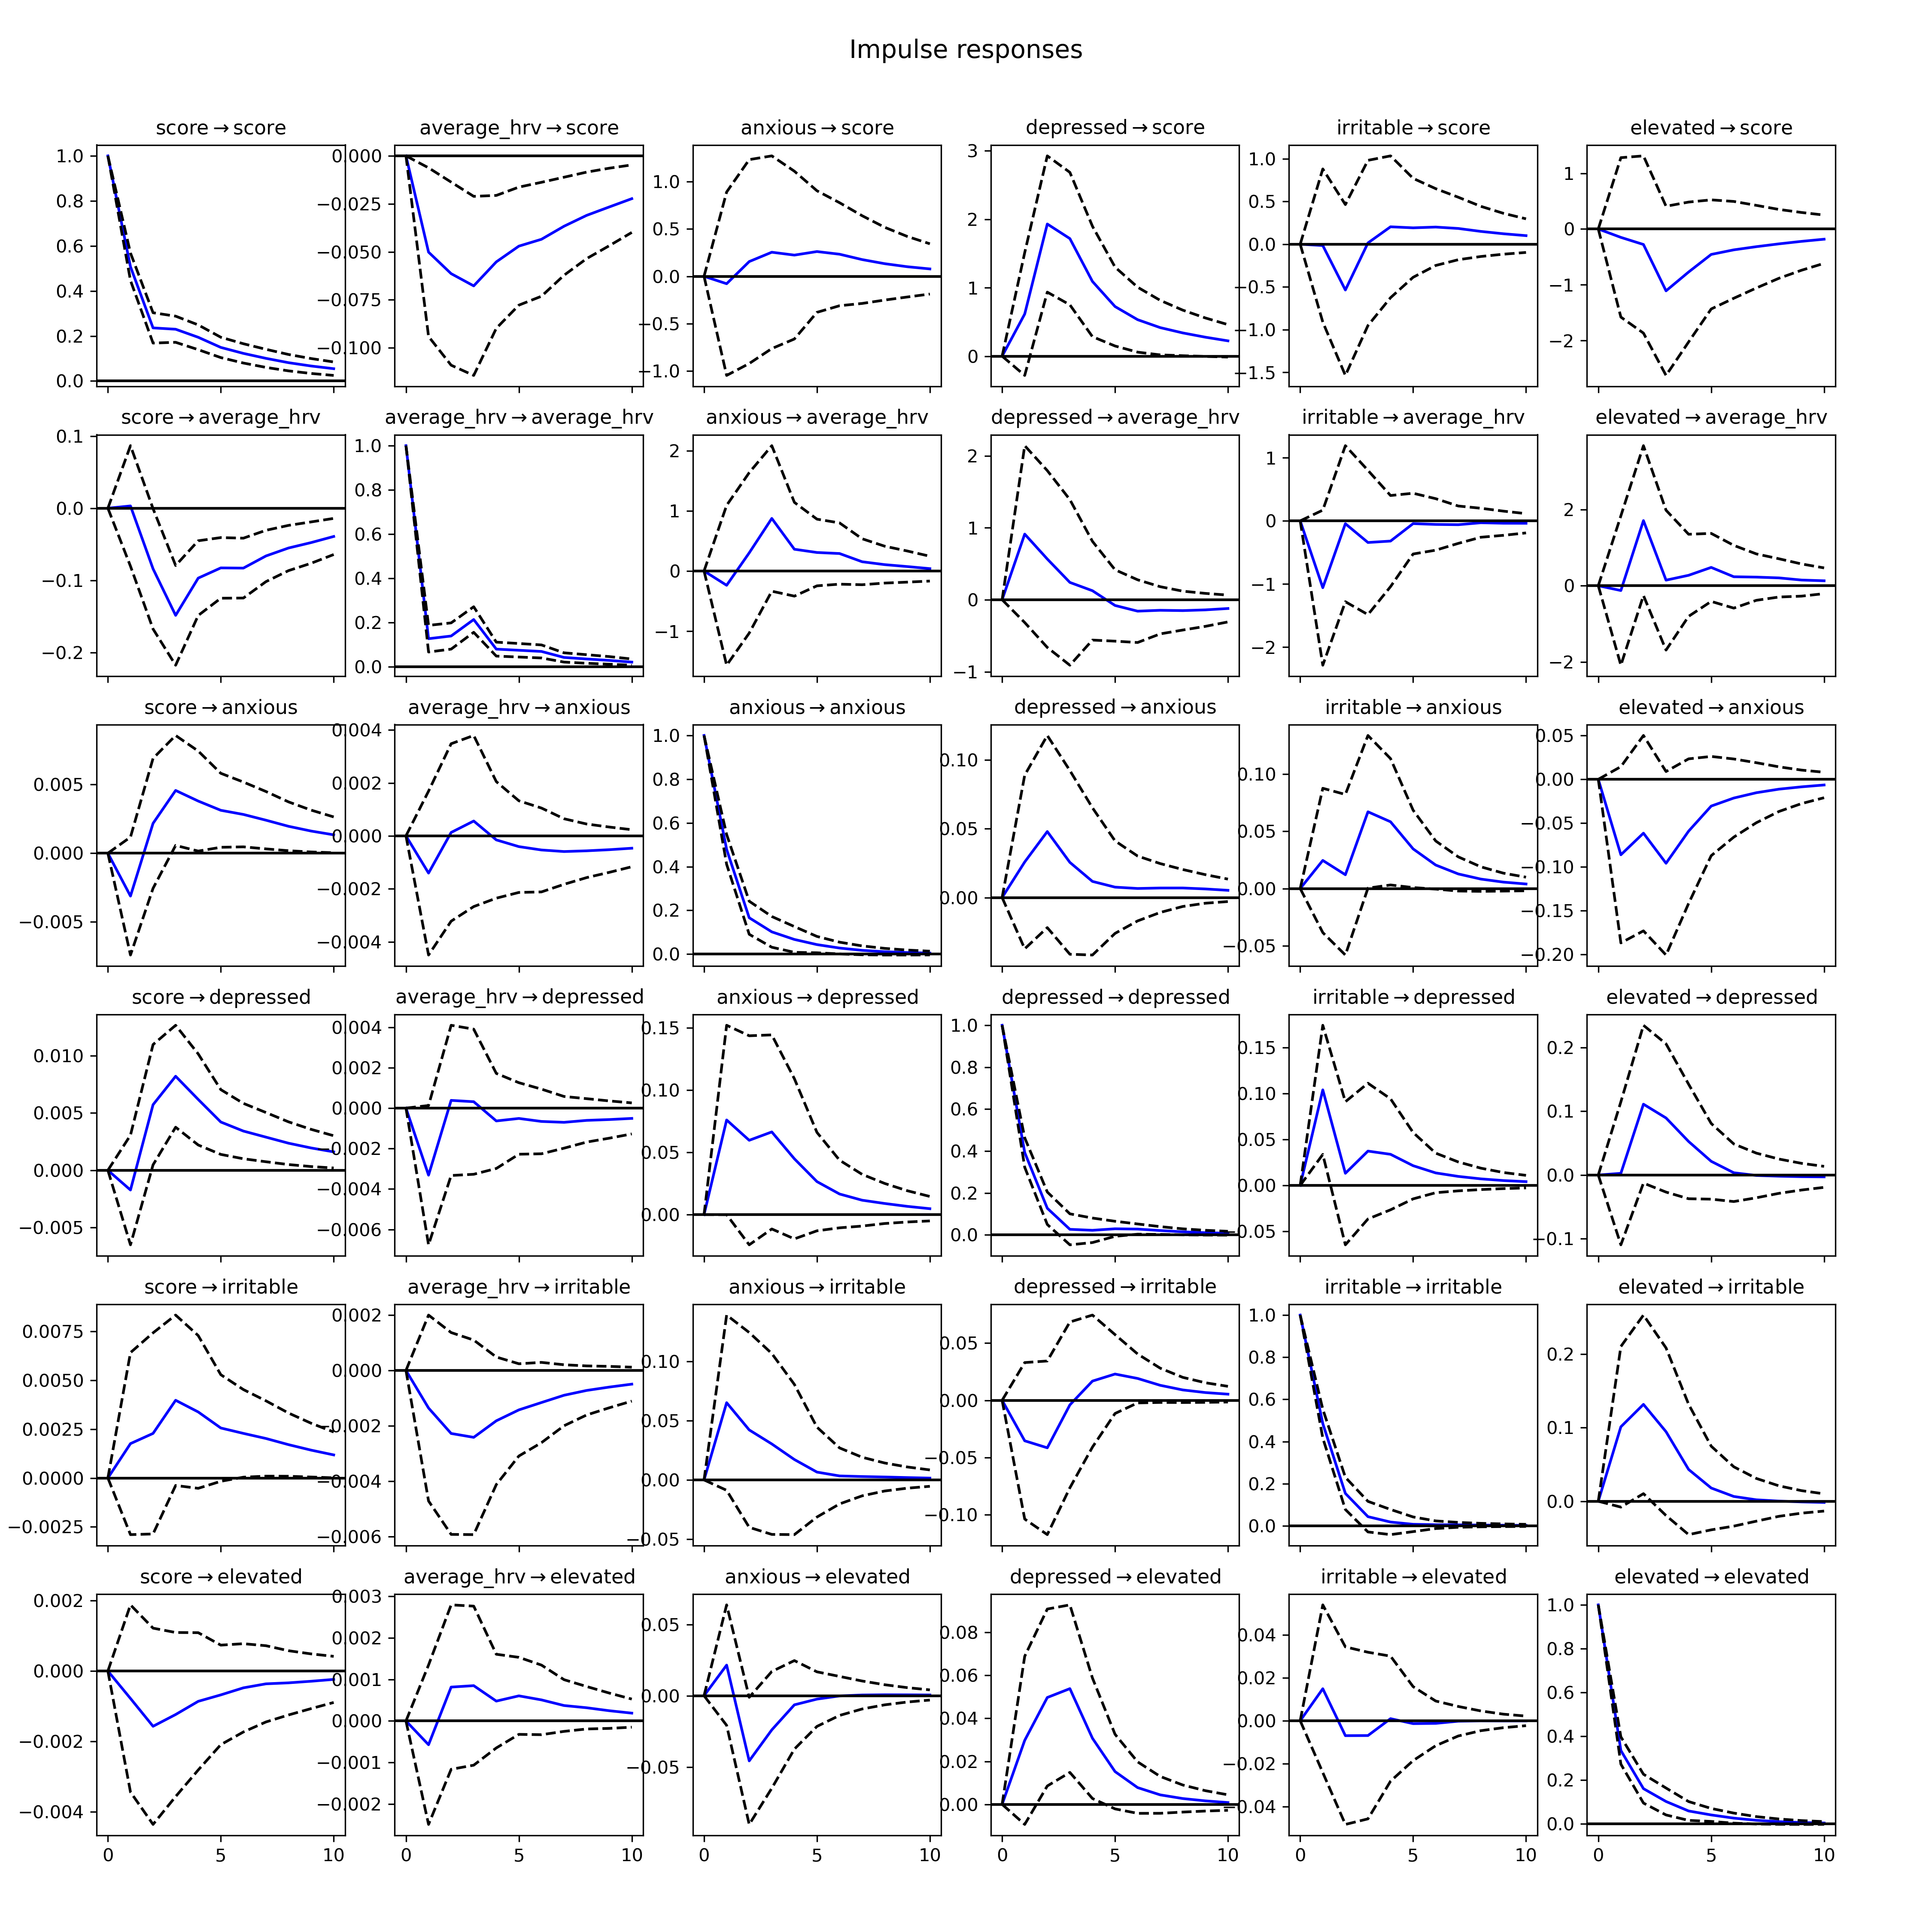
\includegraphics[width=0.9\columnwidth]{/Users/jab/Library/Mobile Documents/com~apple~CloudDocs/PSU/Courses/2023 Spring/STAT508/project/notebooks/plots/IRF_all.png}
  \caption{Plot of Impulse Response Function, Lag 0 to 10}
\end{figure}



\hypertarget{discussion}{%
\section{Discussion}\label{discussion}}

Fusce consectetur accumsan tincidunt. Donec mollis odio at purus
convallis tristique. Phasellus maximus quis tortor quis vehicula.
Vivamus eget aliquam odio. Etiam efficitur feugiat aliquet. Cras sit
amet turpis id nunc interdum placerat. Duis neque nibh, auctor nec
eleifend in, pellentesque eget massa. Duis efficitur urna urna, at
commodo massa efficitur sit amet. Curabitur tincidunt justo sem, sit
amet hendrerit nisi dictum vitae. Ut sed sagittis dolor, vel aliquam
urna. Ut placerat lorem non vehicula vehicula. Pellentesque sed justo
sodales, blandit orci eget, porta sapien.

Donec pellentesque ut ipsum rhoncus venenatis. Aliquam eu nisi vel urna
pharetra mollis. Nulla eget tempus odio. Sed iaculis diam sit amet
accumsan suscipit. Fusce finibus arcu a purus feugiat, at vehicula
sapien venenatis. Etiam fermentum lacus nisl, dictum efficitur enim
fermentum id. Donec accumsan id arcu eu rhoncus. Donec sed magna
posuere, efficitur est eleifend, suscipit nisl. Cras semper sollicitudin
condimentum.

Nulla eleifend eros sodales elit mattis varius vel sed felis. Sed eu
elit ligula. Pellentesque consectetur arcu at tortor hendrerit
venenatis. Praesent luctus dolor eros, mattis pellentesque neque
consectetur eu. Sed iaculis porttitor quam, varius blandit ligula. Sed
justo ante, laoreet in mattis sit amet, fringilla id lectus. Integer
egestas sem ut tortor gravida, a suscipit orci semper.

Nam placerat pellentesque lorem vel iaculis. Aenean congue, nibh ut
mattis pharetra, eros velit mattis enim, consequat rutrum velit justo
sed leo. Curabitur pretium molestie iaculis. Sed malesuada malesuada
nisl nec feugiat. Quisque eu congue erat, id interdum justo. Nam
fringilla condimentum tempus. Ut nec eros hendrerit, pulvinar sapien ac,
molestie nunc. Maecenas mattis ultricies augue, quis lacinia massa
laoreet et. Etiam ut massa vel metus mollis ultrices. Mauris bibendum
neque et lectus vestibulum dapibus. Mauris quis lorem eu est tincidunt
lacinia.

Integer felis massa, rhoncus quis sagittis quis, fringilla non lorem.
Pellentesque feugiat eu nibh eu luctus. Duis faucibus hendrerit justo,
ac condimentum turpis viverra non. Suspendisse egestas et risus sit amet
luctus. In varius quam efficitur nulla efficitur sodales eget in purus.
Quisque sagittis erat nec bibendum eleifend. Integer gravida nibh a
commodo finibus. Nam semper sapien at mauris efficitur pretium.
Phasellus quis egestas nunc.

\bibliography{papers}

\end{document}
